
\section{Numerical implementation}

To solve our optimal control problem we will consider two gradient-based optimization methods \cite{Algorithms}, and compare their performance. We will implement the simpler Gradient Descent method and compare it to Newton's method. The gradient descent method has an infamous slow convergence rate, compared to the super linear convergence rate of Newton's method.

Now since both methods are gradient-based, we need to consider the reduced optimal control problem. Let $S$ be the solution operator for our state system. That is, let $S(u):=\theta(.,T)$ so given a control $u$, $S$ transform the control into the associated final temperature distribution i.e. the solution of the state system at end time. Then we can write our cost functional on reduced form, so our objective become to minimize the reduced cost functional 
\begin{equation}
\label{eq:optimization_prob}
    \min_{u \in U}F(u) := J(S(u),u) = \frac{1}{2}\int_{\Omega}(S(u) - \theta_d)^2 \dx+ \frac{\gamma}{2}\int_0^Tu(t)^2\dt
\end{equation}

The operator S is compact. Now for every $u \in L^2(\Sigma)$ the state system admits a unique solution $\theta \text{ in } L^2(0,T;H^1(\Omega)) \cap C(0,T;L^2(\Omega)$ where $\theta_t \in L^2(0,T;H^1(\Omega)^{*})$. Now due to the bound in Corollary 3.1.1 we have that for every $\delta \in (0,\frac{1}{2})$ there exist a constant $k_{\delta}$ such that 
\begin{equation*}
    ||S(u)||_{H^{\delta}(\Omega)} \leq k_{\delta}||u||_{L^2(\Sigma)} \text{ } \forall u \in L^2(\Sigma)
\end{equation*}
And $H^{\delta}$ embeds compactly into $L^2(\Omega)$ therefore S is indeed compact this argument was taken from \cite{primal_dual}. 


\subsection{Solution of the State- and Adjoint equations}

The state equation and the adjoint equations were both solved numerically with the finite element method, using the finite element programming framework FEniCS \cite{fenics} in python.


\subsubsection{State equation}

For solving the state equation system \eqref{eq:heat} we discretise $\theta$ in time using explicit Euler, so we let
\begin{equation*}
    \theta_t \approx \frac{\theta^{n+1} - \theta^n}{\Delta t}.
\end{equation*}
This is inserted into the equation \eqref{eq:heat-in-omega}. $\theta^{n+1}$ is the unknown, so we set this to just $\theta$. This gives
\begin{equation*}
    \theta - \bar{\alpha}\Delta \theta = \theta^n, \quad\textrm{where}\quad \bar{\alpha} = \alpha\Delta t,
\end{equation*}
and $\alpha$ is the thermal diffusivity defined earlier as $\alpha = \frac{k}{\rho c_p}$. We now multiply with a test function $v\in H^1(\Omega)$, and integrate over the domain, and get
\begin{equation*}
    \int_\Omega \theta v \dx - \bar{\alpha}\int_\Omega \Delta\theta\dx = \int_\Omega \theta^n v\dx.
\end{equation*}
For the implementation it is convenient to combine the two Neumann boundary conditions \eqref{eq:state-system-bd-1} and \eqref{eq:state-system-bd-2} into the following expression
\begin{equation*}
    -k\frac{\partial \theta}{\partial n} = \beta(x)u(t)(\theta - \theta_w) \quad\text{where}\quad \beta(x) = [x\in\Gamma_1],
\end{equation*}
where we have used the Iverson bracket in the definition of $\beta$. Partial integration then lead to the weak form
\begin{equation*}
\begin{aligned}
    \int_\Omega \theta v\dx + \bar{\alpha}\int_\Omega\nabla\theta\nabla v\dx &+ \frac{\bar{\alpha}}{k}\int_{\partial\Omega}\beta(x)u(t)\theta v\ds \\
    &= \int_\Omega\theta^n v\dx + \frac{\bar{\alpha}}{k}\int_{\partial\Omega}\beta(x)u(t)\theta_w v\ds.
\end{aligned}
\end{equation*}
The left hand side, and the left hand side of the weak form above, is a bilinear map, and a linear functional respectively, so we write
\begin{equation*}
    a_S(\theta, v) = L_S(v; \theta^n).
\end{equation*}
In the implementation we set $\theta^0$ using the initial condition given in the system \eqref{eq:heat}, and solve the equation above iteratively forward in time.


\subsubsection{Adjoint equation}

The adjoint system \eqref{eq:adjoint-system} is solved backwards in time. For the time discretisation of $p$ we again use explicit Euler, so we let 
\begin{equation*}
 p_t \approx \frac{p^{n+1} - p^n}{\Delta t}.
\end{equation*}
Since the equation is solved backwards in time, $p^n$ is here the unknown, so we set $p=p^n$, and insert into the adjoint system \eqref{eq:adjoint-system-eqn}. We then get
\begin{equation*}
    p - \bar{\alpha}\Delta p =  p^{n+1}, 
\end{equation*}
% Now multiply with a test function $v\in H^1(\Omega)$ and integrate over the spatial domain to get
% \begin{equation*}
% \int_\Omega pv\dx - \Delta t\frac{k}{\rho c_p}\int_\Omega % \Delta p v \dx = \int_\Omega p^{n+1} v \dx
% \end{equation*}
Again we combine the two Neumann boundary conditions \eqref{eq:adjoint-system-bd-1} and \eqref{eq:adjoint-system-bd-2} into one expression:
\begin{equation*}
    -k\frac{\partial p}{\partial n} = \beta(x)u(t)p,
\end{equation*}
where $\beta$ is as defined above. Now we again multiply with a test function $v\in H^1(\Omega)$ and integrate over the spatial domain. The partial integration then leads us to the weak form
\begin{equation*}
    \int_\Omega pv\dx + \bar{\alpha} \int_\Omega \nabla p \nabla v \dx + \frac{\bar{\alpha}}{k}\int_{\partial\Omega} \beta(x)u(t)pv \ds  = \int_\Omega p^{n+1}v\dx.
\end{equation*}
For the FEniCS implementation we let the left hand side and the right hand side be the bilinear, and linar form respectively, and we thus write
\begin{equation*}
    a_A(p, v) = L_A(v; p^{n+1}).
\end{equation*}
For the implementation we initialise $p^{T/\Delta t}$ using the end time conditions in the adjoint system \eqref{eq:adjoint-system}, and then solve the system above at each time step, backwards in time.


\subsection{Projected Gradient Descent}

The idea of a descent method consist of finding an optimal direction $d_k$ and stepsize $a_k$ at a given iteration $k$, where say our control is given by $u_k$. We want to find
\begin{equation*}
    F(u_k + \alpha_kd_k) < F(u_k)
\end{equation*}

One Taylor expand the LHS around $u_k$ to get a way to choose the descent direction, typically one can take different means to decide this, but a descent direction can in general be chosen by 
\begin{equation*}
    d_k = \arg\min_{||d||_U=1} \langle \nabla F(u_k), d \rangle_U
\end{equation*}
We consider gradient descent therefore we choose the descent direction by setting $d_k = -\nabla F(u_k)$. After deciding the gradient direction one need to determine how far to go in that direction, this is decided by $\alpha_k$, called \textit{line search} parameter. The ideal such parameter is 
\begin{equation*}
    a_k = \arg \min_{\alpha>0} \{ F(u_k + \alpha d_k) \}
\end{equation*}
There are different ways to choose this line search step. One require a couple of properties to be satisfied by this line search parameter these are
\begin{align*}
    F(u_k + \alpha_kd_k) < F(u_k) \text{  } \forall k \\
    F(uk + \alpha_k d_k) - F(u_k) \rightarrow 0 \text{ as } k\rightarrow \infty
\end{align*}
We stick with Armijo rule as our line search strategy. This method consists of given a descent direction $d_k$ of F at $u_k$ choose the largest $a_k \in \{ \beta^0, \beta, \beta^2,..,\beta^m,... \}$ such that
\begin{equation}\label{eq:armijo}
    F (u_k + \alpha_kd_k) - F(u_k) \leq \mu \alpha_k \langle \nabla F(u_k),d_k \rangle_{U}
\end{equation}
where $\mu,\beta  \in (0,1)$ are chosen constant, that is we use backtracking to determine the stepsize \cite{iterativeMethods}. We set $\mu = 10^{-4}$ and $\beta = \frac{1}{2}$. More facts about Armijo rule and the convergence properties of this line search strategy is in \cite{numMethods} \cite{iterativeMethods}. However we have control-constraints, so we need to ensure the argument is placed inside the admissable set of controls $U_{\textrm{ad}}$, in particular we have box constraints given in \eqref{eq:box_constraints}, that is we have a lower bound $u_a$ and upper bound $u_b$ for the control variable. Therefore we need to use a projection onto the set of admissable controls, that is why it is called the projected gradient descent method. We introduce a cut-off function i.e. a projection given by
\begin{equation}
    \label{eq:projection}
    \mathbb{P}_{[u_a,u_b]}(v) := \max \{u_a, \min \{u_b,v \} \}
\end{equation}
this should hold componentwise, if one allow $u_a$ and $u_b$ to be vectors, notation is similar to \cite{Algorithms}. One have to introduce this into the gradient descent method and Armijo's rule. That is we have to consider the projected Armijo's rule which is determine $\alpha_k \in \{1, \frac{1}{2},\frac{1}{4},.. \}$ such that 
\begin{equation*}
    F \bigg (\mathbb{P}_{[u_a,u_b]}(u_k + \alpha_kd_k) \bigg ) - F(u_k) \leq \mu \alpha_k \langle \nabla F(u_k),d_k \rangle_{U}
\end{equation*}
A pseudocode for the whole Projected Gradient Descent method is shown in Algorithm 1. We introduce two stopping criterion's, one based on the minimum allowed step length, and one on the difference in the computed values of the control given by 
\begin{equation}
    \label{eq:stopping}
    \tau := \|u^{(k+1)} - u^{(k)}\|_U 
\end{equation}
This is to check that the controls converge towards a value, $U$ is the space of the controls. We therefore want to consider an optimization algorithm which is based on a quadratic approximation. 

\begin{codebox}
\Procname{$\proc{Algorithm1: Projected Steepest Descent with Armijo}$}
\li Choose initial value $u^{(0)}\in U_{ad}$
\li Set tolerance $\id{tol}$ and $\alpha_{min}$
\li Solve state system to obtain $\theta^{(0)}$, with $u^{(0)}$
\li Solve adjoint system to obtain $p^{(0)}$, with $u^{(0)}$ and $p^{(0)}$
\li $k=0$
\li \While ($\tau > \id{tol}$)  \Then
\li Choose the descent Direction $d_k = -\nabla F(u^{(k)})$
\li Use the Projected Armijo rule to determine $\alpha_k$
\li \If $\alpha_k < \alpha_{min}$ \Then 
\li \textbf{Break} \End
\li Set $u^{(k+1)} = \mathbb{P}_{[u_a,u_b]}\bigg (u^{(k)} + \alpha_k d_k \bigg )$
\li Solve state system to obtain $\theta^{(k+1)}$, with $u^{(k+1)}$
\li Solve adjoint system to obtain $p^{(k+1)}$, with $u^{(k+1)}$ and $\theta^{(k+1)}$
\li Compute $\tau$
\li $k = k +1$
\end{codebox}
This is the projected descent algorithm which we will apply to our control problem. The gradient of our reduced cost functional is given by

\begin{equation*}
    \nabla F(u) =  \gamma u - \frac{1}{\rho c_p} \int_{\Gamma_1} (\theta - \theta_w)p \ds = 0
\end{equation*}

The projected gradient descent method is globally convergent if the reduced cost functional F is Fréchet differentiable and bounded from below. As the solution to the state system $S(u) \in W(0,T) \cap C(\bar{Q})$, $F$ is indeed Fréchet differentiable. Moreover we have that $F(u) \geq 0$ for all choices of controls $u \in U_{ad}$ by the definition of $F(u)$ therefore we have global convergence. However this is a first-order descent method, and the convergence rate is typically very slow, since it solely rely on first-order gradient information. We expect to see pretty fast convergence when the control approximated thus far $u_k$ is far from the optimal, and the convergence gets slower and slower once we get closer to the optimal $\bar{u}$. \bigskip

This behaviour is confirmed by the results shown in figure \ref{fig:armijo}. Here, we first solved the state equation with $u(t) = 1/2$, and used the mean temperature at $t=T$ from this solution as $\theta_d$. We then ran Algorithm 1 (implemented in Python) with initial guess $u^{(0)} = 0.1$, regularisation parameter $\gamma = 1$, minimum allowable normed difference between iterations $\id{tol} = 10^{-10}$ and minimum allowable step length $\alpha_{\min} = 2^{-40}$.\footnote{The values for $\id{tol}$ and $\alpha_{\min}$ are perhaps too small, and could be increased to speed up the algorithm.} The Armijo parameter from \eqref{eq:armijo} was set to $\mu=10^{-4}$. This algorithm reached a value for the control of $0.4903$ after 2 steps, an absolute relative difference of less than 2\% with respect to the correct value of $0.5$. After 9 steps the step length became unacceptably short, and the algorithm terminated with a final value of $u=0.5038$, about 0.8\% away from the correct answer. A complete summary of the values computed by the algorithm are shown in table \ref{table:armijo}. 
\begin{figure}[pb]
    \centering
    \begin{subfigure}[b]{\textwidth}
        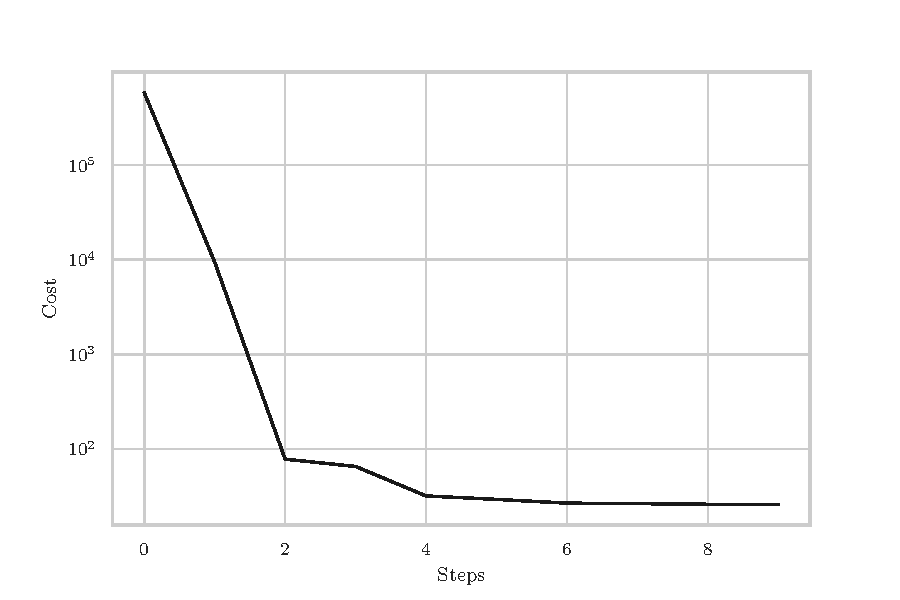
\includegraphics[width=\textwidth]{figures/cost_armijo_analytic_05.pdf}
        \caption{}
        \label{fig:armijo_cost}
    \end{subfigure}
    \begin{subfigure}[b]{\textwidth}
        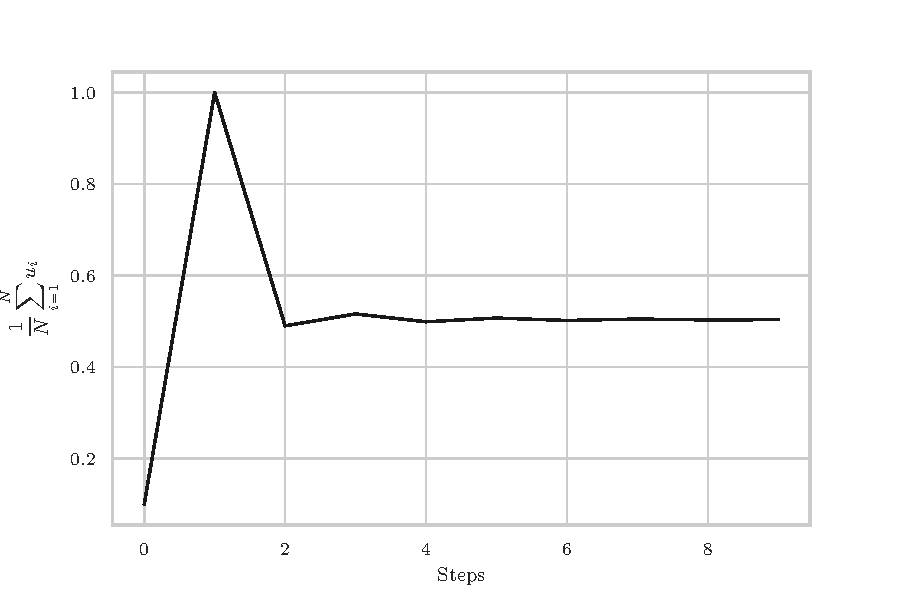
\includegraphics[width=\textwidth]{figures/U_armijo_analytic_05.pdf}
        \caption{}
        \label{fig:armijo_control}
    \end{subfigure}
    \caption{Plots showing (a) the value of the cost-function on a $\log$-scale, and (b) the associated control determined by each step of the Gradient descent algorithm with the Armijo rule. The control used to generate the desired temperature was $u(t) = 1/2$.}
    \label{fig:armijo}
\end{figure}
\begin{table}
    \centering
    \caption{Values computed by Gradient descent with the Arimjo rule.}
    \label{table:armijo}
    \begin{tabular}{@{}lrSS}
         \toprule
    Step ($k$) & Step length ($\alpha$) & \multicolumn{1}{c}{Control ($u^{(k)}$)} & \multicolumn{1}{c}{$\tau = \|u^{(k-1)} - u^{(k)} \|_{\mathcal{U}}$} \\ \midrule
    0 &  & 0.1 &  \\
    1 & $2^{-13}$ & 1.0 & 6.42729 \\
    2 & $2^{-5}$ & 0.49035 & 3.63966 \\
    3 & $2^{-12}$ & 0.5162 & 0.18464 \\
    4 & $2^{-12}$ & 0.49911 & 0.12203 \\
    5 & $2^{-12}$ & 0.5073 & 0.0585 \\
    6 & $2^{-12}$ & 0.50203 & 0.03768 \\
    7 & $2^{-12}$ & 0.50511 & 0.02205 \\
    8 & $2^{-12}$ & 0.50318 & 0.01384 \\
    9 & $2^{-13}$ & 0.50376 & 0.00419 \\ \bottomrule
    \end{tabular}
\end{table}

\subsection{Newton's method}
Another type of direction is obtained at each direction $d_k$ if one instead use a quadratic expansion. For Newton's method we need again the reduced cost function $F$ to be Fréchet differentiable and that its Fréchet derivative is boundedly invertible $\forall u \in U_{ad}$, or at least close to the true solution $\bar{u}$. We try to approximate a solution of the equation $F(u) = 0$ by repeatedly linearizing the function and solving the linearized system
\begin{align}
    \label{eq:Newton}
    u_{k+1} = u_k - F'(u_k)^{-1}F(u_k)
\end{align}
Want to use Newton's method with a primal-dual active set strategy to handle the control constraint. In the unconstrained control case for an optimal control problem, a necessary optimality condition for the reduced control problem is that $\nabla F(u)$ vanishes. However in the presence of control constraints, this condition must be replaced by the variational inequality
\begin{equation}
    \langle \nabla F(\bar{u}), (v-\bar{u}) \rangle \geq 0 \text{ } \forall v \in U_{ad}
\end{equation}
We can reformulate this using Lagrange multipliers, requiring 
\begin{equation*}
    \nabla F(u) + \mu_b - \mu_a =0 
\end{equation*}
to get the complementary slackness conditions which are given by the following equations 
\begin{align}
    \label{eq:complementary}
    \mu_a \geq 0, \quad u_a - u \leq 0, \quad \mu_a(u_a - u) = 0 \\
    \mu_b \geq 0, \quad u - u_b \leq 0, \quad \mu_b(u-u_b) =0
\end{align}
To treat \eqref{eq:complementary} numerically, one combine this into one equation, by introducing a new Lagrange multiplier $\mu = \mu_b - \mu_a$, one convert the complementary slackness conditions into one equation involving maximum and minimum. Therefore the system become 
\begin{align}
    \label{eq:finalComp}
    \nabla F(u) + \mu = 0 \\
    \max \{0, \mu + c(u-u_b) \} + \min \{0, \mu + c(u-u_b) \} - \mu = 0
\end{align}

The latter equation is just a reformulation of the two equations in \eqref{eq:complementary}. Newton's method is based on calculating the Hessian of the reduced cost functional, since it uses second order information about the functional. This depends on the primal variable $u$ and the dual variable $\mu$ we introduce the active and inactive sets at an iterate $(u_k, \mu_k)$ by 
\begin{align}
    \label{eq:active_inactive}
    A_k^{+} := \{ t \in [0,T]: \text{ } \mu_k + c(u_k - u_b) >0 \} \\
    A_k^{-} := \{ t \in [0,T]: \text{ } \mu_k + c(u_k - u_a) <0 \} \\
    I_k := [0,T] \backslash A_k \quad A_k := A_k^{+} \cup A_k^{-}
\end{align}

The Newton direction at an iterate $(u_k, \mu_k)$ can be calculated by solving the following symmetric form of the Newton system

\begin{equation}
    \label{eq:Newton_system}
    \begin{bmatrix}
        \nabla^2 F(u_k) & \chi_{A_k} \\
        \chi_{A_k} & 0 
    \end{bmatrix}
    \begin{bmatrix}
    \delta u \\
    \delta \mu|_{A_k}
    \end{bmatrix}
    = - \begin{bmatrix}
    \nabla F(u_k) + \mu_k \\
    \chi_{A_k^{+}}(u_k - u_b) + \chi_{A_k^{-}}(u_k - u_a)
    \end{bmatrix}
\end{equation}
The next dual variable $\mu_{k+1}$ is set to be zero on the the inactive set $I_k$. A Pseudocode for Newton's method with primal-dual active set strategy is given in Algorithm 2

\begin{codebox}
\Procname{$\proc{Algorithm2: Newton's method with Primal-Dual Active Set Strategy}$}
\li Choose initial value $u^{(0)}$ and $\mu_0$ 
\li Set tolerance $tol$
\li Set $k = 0$
\li Solve state system to obtain $\theta^{(0)}$
\li Solve adjoint system to obtain $p^{(0)}$
\li \While $(\tau > \id{tol})$ \Then 
\li Evaluate the reduced gradient $\nabla F(u_k)$
\li Compute the active sets $A_k^{+}$ and $A_k^{-}$
\li \If $A_k^{+} = A_{k-1}^{+}$ and $A_{k-1}^{-} = A_k^{-}$ \Then 
\li \textbf{break} \End
\li Solve the Newtonian system given in \eqref{eq:Newton_system} iteratively
\li $u^{(k+1)} = u^{(k)} + \delta u$  
\li \If $t \in A_k$ \Then
    \li $\mu_{k+1} = u_k + \delta u$
    \li \Else $\mu_{k+1} = 0$ 
    \End
%\begin{equation*}
%    \mu_{k+1}(t) = 
%    \begin{cases}
%     u_k + \delta u \text{ if } t \in A_k \\
%     0 \qquad \text{ if } t \in I_k
%     \end{cases}
% \end{equation*}
\li Solve state system to obtain $\theta^{(k+1)}$ using $u^{(k+1)}$
\li Solve adjoint system to obtain $p^{(k+1)}$ 
\li Compute $\tau$
\li $k = k+1$
\end{codebox}

Where $\tau$ is calculated as in Algorithm 1.  Numerical experiments show that algorithm is rather insensitive to the initial control $u_0$  \cite{primal_dual}. In the article by Kunish and Rösch \cite{primal_dual} it is proven that when the algorithm satisfy the stopping criteria in step 9, then the last iterate produced $(u_n, \theta_n, p_n, \mu_n)$ satisfy the optimality system for the original optimal control problem. Furthermore a convergence analysis of the algorithm is carried out in the same article. Now the practical behaviour for some active set stragies is that the controls computed in the iterations are infeasible, except for the last iteration which is feasible. By the argument in \cite{primal_dual} the algorithm stops at a feasible and optimal point. The algorithm can be made more efficient by for instance carrying out a few gradient descent steps in the starting phase, and then switching over to Newton's method. The notion used here is similar to that in \cite{Algorithms}. \bigskip

Expect to observe superior convergence properties of Newton's method compared to Steepest Descent, as Newton's method is superlinearly convergent compared to $q$-linearly convergent. The rate of convergence can be measured similarly as in \cite{DPSteel} by setting 
\begin{equation}
    \label{eq:rate_of_conv}
    e_k := \frac{||u^{(k)}-\bar{u}||_U + ||\theta^{(k)}-\bar{\theta}||_{L^2(Q)} +||p^{(k)}-\bar{p}||_{L^2(Q)} }{||u^{(k+1)}-\bar{u}||_U + ||\theta^{(k+1)}-\bar{\theta}||_{L^2(Q)} +||p^{(k+1)}-\bar{p}||_{L^2(Q)}}
\end{equation}
where $(\bar{\theta},\bar{u},\bar{p})$ is the analytical solution to the control problem. We use this as a convergence test of the two algorithm on a control problem where we can find an analytical solution. 

Other mentionable methods to use on the optimal control problem is the sequential quadratic programming (SQP) method \cite{Algorithms}, and reduced SQP \cite{DPSteel}. 
